% Dokumentation von Julian Sehbaoui%

%Set the documentclass to article with a4 paper and 10pt font%
\documentclass[a4paper, 10pt]{scrartcl}

%importing german packages%
\usepackage[ngerman]{babel}
\usepackage[utf8]{inputenx}
\usepackage[T1]{fontenc}

%importing the other packages%
\usepackage{amsmath}
\usepackage{xcolor}
\usepackage{hyperref}
\usepackage{listings}
\usepackage{enumerate}
\usepackage{graphicx}
\usepackage{fancyhdr}
\usepackage{sidecap}
\usepackage{placeins}
\usepackage{wrapfig}
\usepackage[export]{adjustbox}
\usepackage{tikz-uml}
\usepackage{verbatim}
\usepackage{lastpage}
\usepackage{setspace}
\usepackage{biblatex}

\sidecaptionvpos{figure}{t}

%setting the listing package settings for later code blocks%
\lstset{frame=tb,
  language=Python,
  aboveskip=3mm,
  belowskip=3mm,
  showstringspaces=false,
  columns=flexible,
  basicstyle={\small\ttfamily},
  numbers=none,
  numberstyle=\tiny\color{gray},
  keywordstyle=\color{blue},
  commentstyle=\color{green},
  stringstyle=\color{purple},
  breaklines=true,
  breakatwhitespace=true,
  tabsize=3
}

%creating the header and footer%
\pagestyle{fancy}
\fancyhf{}
\lhead{Julian Sehbaoui}
\chead{\glqq Schach.py\grqq{}}
\rhead{Luisen-Gymnasium Bergedorf}
\cfoot{\thepage\ von \pageref*{LastPage}}
\renewcommand{\headrulewidth}{2pt}
\renewcommand{\footrulewidth}{1pt}

%setting document attributes for the titlepage%
\title{Informatik Dokumentation \glqq Schach.py\grqq}
\author{Julian Sehbaoui S4 MINT}
\date{\today}

\parindent 0pt

\bibliography{refs.bib}

%begin the document
\begin{document}

%create the titlepage%
\begin{titlepage}
        \maketitle
        \centering
        \Large
        Besondere Lernleistung: Fachbereich Informatik
        \normalsize
        \doublespacing
        \url{https://github.com/JSehbaoui/Chess_Python}\\
         \vspace{5pt} 
        \includegraphics[scale=0.35]{assets/luisengymnasium.png}\\
         \vspace{5pt} 
        
        Made with \LaTeX{}
\end{titlepage}

%creating a single page just for the table of contents%
\pagebreak
\tableofcontents
\pagebreak

%THE DOCUMENTATION:%
\section{Vorwort}
Dieses Projekt findet im Rahmen des Informatikunterrichts des Luisengymnasiums 	Bergedorf statt und wird als zusätzliche Lernleistung entsprechend gewertet.
Ich bin Julian Y. Sehbaoui und habe ein Schachprogramm „from scratch“ in Python 3 geschrieben.

\section{Mein Ziel}
Mein Ziel war es, ein vollfunktionales Schachspiel ausschließlich in Python 3
zu erschaffen, welches alle klassischen Regeln von Schach beinhaltet. 
Hierbei wollte ich auf jegliche äußerliche Hilfe, wie zum Beispiel API's oder schon
existierende Algorhytmen, verzichten, mit Ausnahme eines Schachcomputers, gegen den man spielen kann. 
Außerdem soll man zwischen PvP\footnote{Player versus Player} und PvE\footnote{Player versus Enviroment} wählen können,
um das Endprodukt entweder mit Freunden oder auch alleine benutzen zu können.

\section{Ideenfindung}
Ich persönlich habe mich schon seit dem ich klein war für Schach interessiert.
Es ist ein Spiel mit relativ simplen Regeln, welches aber durch seine zahlreichen Zugmöglichkeiten schnell sehr komplex werden kann.
Als ich mich nach einem neuen Projekt umgesehen habe, kam mir direkt Schach in den Sinn, weil es an strikte Regeln gebunden ist und
ich zu dem Zeitpunkt dachte, dass wenige Sonderregeln existieren.
Außerdem wollte ich mich immer weiter vom Terminal entfernen und mehr mit
GUI's\footnote{Graphical User Interfaces} arbeiten. Ein weiterer Grund für meine Entscheidung war,
dass mir Schach als Herausforderung in den Sinn kam, um meine aktuellen Fertigkeiten
unter Beweiß zu stellen und mich selbst zu fordern.

Außerdem wollte ich eine Offline Schachversion für meinen Laptop haben
damit ich nicht immer zu einer webbsierten Version zurückgreifen muss. Da mir aber die
Alternativen nicht gefielen, habe ich mich an meine eigene Version gemacht. Sie sollte
alles können, was die Onlinespiele können, also die Basisregeln beachten und eine benutzerfreundliche
Oberfläche bieten. 

\section{Warum Schach?}
Warum schreibe ich mein eigenes Schachprogramm, wenn es diese zuhauf online gibt und die meisten Versionen kostenlos sind?
Zu nächst wollte ich mich wie bereits erwähnt mit einem neues Projekt fordern und vorallem mich mit GUI's vertraut machen.
Zum anderen gibt es Features, die ich gerne bei der \glqq Konkurenz\grqq{} gesehen hätte, zum Beispiel den Testmodus (später erläutert).

\section{Die Regeln im Schach}
Die Regeln des modernen Schachspiels sind dokumtentiert und online abrufbar\cite{schachregeln}.

\section{Benutze Pakete}
Im Folgenden finden sich die verwendeten Pakete sowie deren Vorteile, welche mich zu der Entscheidung geführt haben.

\subsection{pygame}
\glqq pygame\grqq{}~\cite{pygame} ist eine Ansammlung von Python 3-Modulen, welche auf das programmieren von Videospielen ausgelegt sind. Es ist auf sämtlichen OS verfügbar und hat schon mehrere Millionen Benutzer.

\subsubsection*{Warum pygame?}
\glqq pygame\grqq{} ist aufgrund der großen Community sehr gut dokumentiert.
Außerdem basiert es auf SDL~\cite{SDL}, was eine gute Input-Abfrage ermöglicht.
Ein weiterer Grund für die Verwendung von \glqq pygame\grqq{} war, dass ich schon ein
wenig Erfahrung mit dem Modul sammeln konnte und daher für mich die erste
oberflächliche Benutzung erleichtert wurde.
Eine Alternative für mich war die \href{https://processing.org/}{\color{blue}{\glqq Processing\grqq}}.
\glqq Processing\grqq{} ist ein \glqq Sketchbook \grqq{} , welches einem erlaubt,
auf einer graphischen Oberfläche zu programmieren. Es ist ein leichtverständliches
Prinzip, da man hier mit der Syntax von entweder Java oder Python 3 funktionell programmieren
kann. Außerdem, da Processing für graphische Arbeiten und kleine Spiele geschaffen wurde,
lässt sich schnell und einfach die Mausposition und weitere Inputs abfragen und
Figuren und Bilder auf der graphischen Oberfläche abbilden.
Der Grund, warum ich mich dennoch für \glqq pygame\grqq{} entschieden habe, war, dass man in \glqq pygame\grqq{}
objektorientiert~\cite{OOP} arbeiten kann. Dieses Konzept ist hilfreich bei der Programmierung eines Schachspiels,
da sich alle Figuren an den selben \glqq Bauplan\grqq{}  halten und über das Prinzip der Vererbung
die figurtypischen Eigentschaften in dieses Grundgerüst implementieren lassen.

\subsubsection*{Was habe ich verwendet?}
Von dem Paket \glqq pygame\grqq{} habe ich die \glqq Display\grqq{}-Methode benutzt, welche das Fenster erstellt hat. Außerdem habe ich
die Funktion \glqq draw\grqq{} benutzt, um Formen, wie zum Beispiel die einzelnen Quadrate des Bretts, Bilder, wie zum Beispiel die der Figuren,
und Schriftzüge auf das Display zu bringen. Ebenfalls hilfreich war die Klasse \glqq Surface\grqq , mit der man einzelne kleine Bereiche abgrenzen konnte,
um so mehr Struktur in das GUI zu bringen.  

\subsection{pygame-widgets}
\glqq pygame-widgets\grqq{} ist eine Art Erweiterung für \glqq pygame\grqq , welche Klassen für zum Beispiel Buttons und Schieberegler mitsich bringt.

\subsubsection*{Warum pygame-widgets}
Die Erweiterung war sehr hilfreich, da ich somit einzelne Widgets nicht selber schreiben musste.

\subsubsection*{Was habe ich verwendet?}
Von \glqq pygame-widgets\grqq{} habe ich nur den Schieberegler für die Anpassung der Computerschwierigkeit verwendet. Obwohl ich Buttons verwendet
habe, programmierte ich diese selber, da ich so viel mehr Freiheit hatte, was Funktion und Design anging. Für den Schieberegler hingegen
war das Paket jedoch ausreichend, weswegen ich mir die Arbeit des Selberschreibens hier gespart habe.

\subsection{Stockfish}
\glqq Stockfish\grqq~\cite{Stockfish} ist eine berühmte Schachengine, welche von vielen großen Schachanalysten und Schachwebsites, wie zum Beispiel \url{lichess.org} oder \url{chess.com}, benutzt wird.

\subsubsection*{Warum Stockfish?}
Auf der Suche nach einer Schach-KI hatte ich gewisse ansprüche.
\begin{enumerate}
        \item Die KI braucht eine Python 3-Unterstützung
        \item Der Service soll nicht über eine API laufen, da ich das Spiel auch
        offline benutzen möchte
        \item Die KI muss Open-Source sein.
\end{enumerate}
Von meinen bisherigen Schacherfahrungen aus der Vergangenheit blieb mir
der Name \glqq Stockfish\grqq{} im Kopf. Als ich recherchierte sah ich, dass die 
\glqq Stockfish\grqq{}-Engine nicht nur Open-Source ist, sondern sogar in pip\footnote{\textbf{P}ackage \textbf{I}nstaller for \textbf{P}ython} vorhanden war.
Somit hatte \glqq Stockfish\grqq{} alle meine Anforderungen erfüllt und ich hatte keinen Grund mehr,
nach Alternativen zu suchen.
Zudem ist \glqq Stockfish\grqq{} sehr populär unter den Schachspielern, weswegen ich mir eine
gute Dokumentation erhoffte.\\
Alternativen zu \glqq Stockfish\grqq{} wären noch Alpha Zero\footnote{Eine Schach-KI von Google}
sowie viele kleine selbstgeschriebene Engines. Jedoch überzeugte \glqq Stockfish\grqq{} auch mit
seiner hervorragenden Informationsübermittlung, da man zur Kommunikation zwischen
meinem Skript und \glqq Stockfish\grqq{} nur das Format geringfügig ändern musste und schon funktionierte
die Engine einwandfrei.  

\subsubsection*{Was habe ich verwendet?}
Von Stockfish habe ich die Klasse \glqq Stockfish\grqq{} verwendet. 
Von dieser wiederum habe ich die Methode \glqq get\_best\_move\grqq{} verwendet,
um einen legalen und taktisch sinnvollen Zug für den Computer zu ermitteln. 


\section{Installation}
Mein Skript kann kostenlos von der Seite \href{https://github.com/Aetherion-dot/Chess_Python}{\color{blue}{github}} herutergeladen werden.
Natürlich muss man, um das Python 3-Skript auszuführen, \href{https://www.python.org/downloads/}{\color{blue}{python3}} installiert haben.
Hierbei ist jede Version von Python 3 möglich, jedoch arbeitete ich mit Python 3.8.X, weswegen ich diese Version empfehlen würde.
Um dieses dann zu starten sind die Pakete „Stockfish“, „pygame“ und "pygame-widgets" über \href{https://pypi.org/project/pip/}{\color{blue}{pip}} herunterzuladen.
Dies ist über die Konsole mit den Befehlen
\begin{lstlisting}[language=bash]
        pip install pygame
\end{lstlisting}
\begin{lstlisting}[language=bash]
        pip install stockfish
\end{lstlisting}
\begin{lstlisting}[language=bash]
        pip install pygame-widgets
\end{lstlisting}
zu erreichen.
\pagebreak
\section{Bedienung des Programmes}
Im Folgenden erläutere ich die Bedienung des Programmes.
\subsection{Wie spiele ich?}
Um das Schachprogramm zu starten, muss man die \glqq start.py\grqq{}-Datei in Python 3 starten. Anschließend öffnet sich ein Fenster, in welchem man zwischen verschiedenen Spielmodi
wählen kann.

\begin{figure}[h]
        \centering
        \includegraphics[width=0.4\textwidth]{assets/start_screen.PNG}
        \caption{Startbildschirm \textit{(Eigenaufnahme)}}
\end{figure}
Die beiden Modi, die hier zur Auswahl stehen, sind einmal die Standard-Schach-Variante und die Chess 960 Variante~\cite{chess960},
bei der die Figuren in der hinteren Reihe zufällig angeordnet werden.
Für jeden der beiden Modi lässt sich optional ein zweiter, virtueller Spieler hinzufügen, falls man keinen realen Gegner bei sich hat.
Das kann durch das Klicken des grauen Feldes neben der Nachricht \glqq{}Play against AI\grqq{} erreicht werden.
Nachdem man sich für einen Modus entschieden hat, lässt sich der Spielername, und je nach Option die Computerschwierigkeit oder der Name des zweiten Spielers, einstellen.
\begin{figure}[!h]
        \centering
        \begin{minipage}[b]{.4\linewidth} % [b] => Ausrichtung an \caption
           \includegraphics[width=\linewidth]{assets/login_w_bot.PNG}
           \caption{Modus mit Bot \textit{(Eigenaufnahme)}}
        \end{minipage}
        \hspace{.1\linewidth}% Abstand zwischen Bilder
        \begin{minipage}[b]{.4\linewidth} % [b] => Ausrichtung an \caption
           \includegraphics[width=\linewidth]{assets/login_wo_bot.PNG}
           \caption{Modus ohne Bot \textit{(Eigenaufnahme)}}
        \end{minipage}
\end{figure}

Nun kann das Spiel durch den Knopf unterhalb der Einstellungen gestartet werden und das tatsächliche Spiel kann beginnen.
Sobald man auf eine Figur klickt, öffnen sich auf dem Feld alle legalen Zugoptionen.

\begin{figure}[h]
        \centering
        \includegraphics[width=0.5\linewidth]{assets/Spielbrett_pawn.PNG}
        \caption{Das Spielbrett nach klicken auf e2}
\end{figure}
Wenn man anschließend auf ein Feld klickt, welches die Figur betreten kann, bewegt
sich die ausgewählte Figur auf das gewünschte Feld.

\subsection{Overlays}

\subsubsection*{Spielerinformationstabs}
Im oberen Bereich des Spielfelds befindet sich zum einen eine Uhr, welche die aktuelle Spielzeit anzeigt. Links und rechts danaben befinden sich die Spielerinformationen.

\begin{figure}[h]
        \centering
        \includegraphics[scale=0.7]{assets/infotabs.PNG}
        \caption{Informations-Tabs und Spielzeit}
\end{figure}
In diesen werden die geschlagenen Figuren sowie der Spielername angezeigt. Außerdem wird das Spielerinformationsfeld von dem Spieler hervorgehoben, welcher an der Reihe ist, den
nächsten Zug zu machen.

\subsubsection*{Spielhistorie}

In dem rechten Teil des Fensters befindet sich die Spielhistorie.
Diese zeigt die bereits gezogenen Spielzüge in der \glqq Ausführlichen Notation\grqq{} an. 

\subsubsection*{Buttons}
In der rechten, oberen Ecke finden sich insgesammt vier Buttons mit folgenden Funktionen:
\begin{wrapfigure}{r}{0.5\textwidth}
        \centering
        \vspace{48mm}
        
\includegraphics{assets/Buttons.PNG}
        \caption{Bedienungs-Knöpfe}
\end{wrapfigure}

\begin{itemize}
        \item \glqq Quit\grqq-Button
        \begin{itemize}
                \item Der Quit-Button beendet sofort das Spiel und schließt das Fenster
        \end{itemize}
        \item \glqq Resign\grqq-Button
        \begin{itemize}
                \item Beendet das Spiel mit einem Sieg für den anderen Spieler
        \end{itemize}
        \item \glqq Takeback\grqq-Button
        \begin{itemize}
                \item Macht den letzten Zug rückgängig
                \item Ist nur zu benutzen, wenn keine Figur im 
                letzten zug geschlagen wurde, um große Patzer zu bestrafen
        \end{itemize}
        \item \glqq Testmodus\grqq
        \begin{itemize}
                \item Bei erstmaligem Drücken betritt man einen Testmodus, indem es einem möglich
                einem möglich ist, Züge auszutesten.
                \item alle Züge revidiert und die Figuren
                auf ihre Ausgangsposition zu beginn des Testens zurückgestellt 
        \end{itemize}
\end{itemize}


\pagebreak
\section{Code}
In dem folgenden Kapitel werde ich das Konzept meines Codes erläutern und die Entwicklung darstellen. 


\subsection{Klassenbeziehungen}

\begin{figure}[!h]
\begin{center}
\resizebox*{.7\textwidth}{.75\textheight}{%
\begin{tikzpicture}
%\begin{umlpackage}{Chess}
\begin{umlpackage}{Figuren}
\umlclass{Pieces}{
	master : pygame.Surface \\ 
	name : String \\
	tile x : int \\
	tile y : int \\
	color : Tuple \\
	image : pygame.image \\
	value : int 
}{
        draw() : void \\
        animate() : void \\
        move() : void \\
        foresight() : bool \\
}
\umlclass[x=-3,y=-5]{BlackPawn}{}
{
        getPossibleMoves() : array \\
        promotion() : void \\
        attacked\_tiles : array
}
\umlclass[x=3,y=-5]{WhitePawn}{}
{
        getPossibleMoves() : array \\
        promotion() : void \\
        attacked\_tiles : array
}
\umlclass[x=-3,y=-7.5]{Knight}{}
{
        getPossibleMoves() : array \\
        attacked\_tiles : array
}
\umlclass[x=3,y=-7.5]{Bishop}{}
{
        getPossibleMoves() : array \\
        attacked\_tiles : array
}
\umlclass[x=-3,y=-10]{Rook}{}
{
        getPossibleMoves() : array \\
        attacked\_tiles : array
}
\umlclass[x=3,y=-10]{Queen}{}
{
        getPossibleMoves() : array \\
        attacked\_tiles : array
}
\umlclass[x=0,y=-12.5]{King}{}
{
        getPossibleMoves() : array \\
        attacked\_tiles : array
}
\umlinherit[geometry = |-]{Pieces}{WhitePawn}
\umlinherit[geometry = |-]{Pieces}{BlackPawn}
\umlinherit[geometry = |-]{Pieces}{Knight}
\umlinherit[geometry = |-]{Pieces}{Bishop}
\umlinherit[geometry = |-]{Pieces}{Rook}
\umlinherit[geometry = |-]{Pieces}{Queen}
\umlinherit{Pieces}{King}

\end{umlpackage}

\end{tikzpicture}
}
\caption{UML-Diagram der Figurenklassen}
\end{center}
\end{figure}
Oben zu sehen ist ein UML-Diagramm, um die Beziehungen von den verschiedenen
Klassen zu visualisieren. Zu erkennen ist eine Parentclass \glqq{}Pieces\grqq ,
welche alle Methoden enthällt, die für eine beliebige Schachfigur von nöten sind.
Von dieser Klasse erben insgesammt sieben andere Klassen. Jede Klasse hat ihre eigene
Methode, um die möglichen Züge zu berechnen. Getrennt sind hierbei die Bauern, in
\glqq BlackPawn\grqq{} und \glqq WhitePawn\grqq{}. Das ist nötig, da sich die Bauern der verschiedenen Teams als
einzige Figur nicht exakt so wegbewegt, wie die des gegnerischen Teams. So bewegt sich
der weiße Bauer aufsteigend der Reihen, wohingegen sich der schwarze Bauer absteigend der
Reihen bewegt. 

\subsection{Probleme und Problemlösungen}
Während des Programierens bin ich auf viele Probleme gestoßen, die mich an meine Grenzen gebracht haben, welche ich aber immer wieder überwinden konnte.
Das wohl größte Problem war, dass viele Regeln Voraussetzungen mit sich bringen, die man beim normalen Spielen gar nicht aktiv bedenkt, welche aber
beim Implementieren eine Hürde darstellten.

\subsubsection*{Das Verrücken des Spielbretts}
Als ich grob mit dem Aufbau meines Schachprogramms
fertig war, also die Figuren, welche sich noch ohne
Einschränkungen bewegen konnten, auf einem richtig koloriertem
Feld standen, wollte ich das Schachbrett verrücken, um Platz für
die zukünftigen Overlays zu schaffen.
Die ersten Versuche hatten zur Folge, dass die Figuren nicht mehr auf die
Events, wie zum Beispiel einen Mausklick, reagierten.\\
Als das Problem behoben war, traten aber viele visuelle Probleme auf.

\begin{figure}[h]
        \centering
        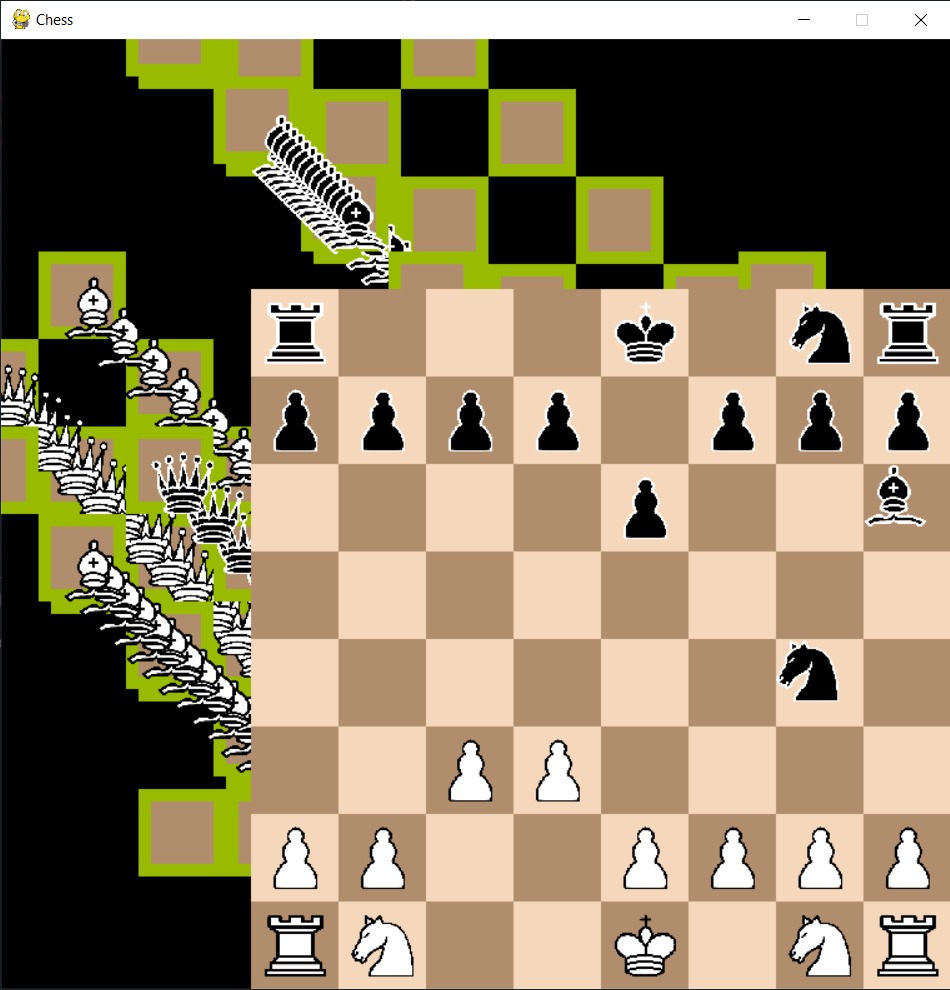
\includegraphics[scale=0.3]{assets/tf_have_I_done.png}
        \caption{Graphischer Fehler}
\end{figure}
Das Problem ließ sich durch die weiteren Einschränkungen
der Bewegungsfreiheit der Figuren, sowie das Hinzufügen eines
Anker-Punktes an der oberen-rechten Ecke des Spielbretts beheben. 


\subsubsection*{Der König, das Problemkind}
Das wohl größte Problem war der König. Dieser muss nämlich, abhängig von der Stellung des Bretts,
in seinen Bewegungen eingeschränkt werden. Die Lösung der Felderbegrenzung konnte durch einen simplen Filter gelöst werden. Das erste, große Problem kam nun aber mit dem
Blocken eines Schachs. Wenn eine Figur zwischen König und der angreifenden Figur steht, dann ist das Schach aufgelöst. Nur was bedeutet nun \glqq{}dazwischen \grqq?
Um dieses Problem zu lösen, musste ich den König entlang der Angriffslinien \glqq{}tracken\grqq{}. Als ich nach langer Zeit das Problem gelöst hatte, kam nun leider ein weiteres Problem hinzu. 
Der König konnte sich selbst blockieren bzw. das Schach im nächsten Zug verhindern, was wie folgt aussah: 
\begin{figure}[!h]
\centering
\includegraphics[scale=0.6]{assets/Bug_king_blocking.png}
\caption{Bug, König verhindert Schach}
\end{figure}\\
Um dieses Problem zu lösen, hatte ich erst die Idee, den König zu einer \glqq{}transparenten
Figur\grqq{} zu machen, sodass der Angriffszug auch durch diesen hindurch geht. 
Als ich jedoch dabei war die dieses Problem zu lösen, taten sich viele weitere Bugs auf, wie zum Beispiel, dass man die 
Figur, die vor dem König steht und das Schach verhindert wegbewegt werden darf, obwohl das kein legaler Zug ist.
Aufgrunddessen suchte ich nach einer Lösung, welche alle nicht-legalen Züge verhindern würde.

\subsubsection*{Foresight}
Wenn man es schaffen könnte, nach dem nächsten Zug in die Zukunft zu sehen und erkennen könnte, ob
der Zug als Konsequenz hat, dass der König im Schach steht, könnte man diesen Zug verbieten. 
Genau das war der Gedanke hinter dieser Lösung. Ich lasse, bevor ich die möglichen Züge
einer Figur exportiere, die Liste durch einen Filter laufen, der oben Erwähntes prüft.
Der Filter sieht folgendermaßen aus:

\begin{lstlisting}
def filter_method_foresight(self, move):
        self.x, self.y = move #setting the position of the piece to the move, that you want to check
        ignoring_piece = None #currently no piece has to be ignored

        ### if you want to simulate to take a piece, 
        # without actually taking it, you can just 
        ### ignore it in the .detectingCheck method
        same_pos = (self.x, self.y) == (piece.x, piece.y)
        same_piece = piece == self
        for piece in Pieces.all_pieces_list:
                if same_pos and not same_piece:
                        ignoring_piece = piece

        #checking if the king is checked, after the move
        Pieces.detectingCheck(ignoring_piece = ignoring_piece)

        white_check = bool(Pieces.white_is_checked)
        black_check = bool(Pieces.black_is_checked)
        white = bool(self.farbe == (255,255,255))
        black = bool(self.farbe == (0,0,0))

        #returning if the move is legal or not
        return (white and not white_check) or (black and not black_check)
\end{lstlisting}
Nachdem ich diesem Filter für jede Figur angewendet hatte, gab es keinerlei Probleme mehr mit
illegalen Zügen. 

\pagebreak
\subsubsection*{Stockfish}
Vorerst glaubte ich noch an die Einfachheit der Implementierung von Stockfish in
Python 3, aber diese Vermutung erwies sich als falsch. Zunächst habe ich Stockfish wie in
der Dokumentation beschrieben installiert und importiert. Als ich dann ein Objekt der
Klasse \glqq Stockfish\grqq{} erstellen wollte, bekam ich folgende Fehlermeldung:
\begin{lstlisting}
        Traceback (most recent call last):
        File "D:\Julian\Coding\Sprachen\python\lib\site-packages\ stockfish\models.py", line 33, in __init__
        self.stockfish = subprocess.Popen(
        File "D:\Julian\Coding\Sprachen\python\lib\subprocess.py", line 947, in __init__
        self._execute_child(args, executable, preexec_fn, close_fds,
        File "D:\Julian\Coding\Sprachen\python\lib\subprocess.py", line 1416, in _execute_child
        hp, ht, pid, tid = _winapi.CreateProcess(executable, args,
        FileNotFoundError: [WinError 2] Das System kann die angegebene Datei nicht finden
        Exception ignored in: <function Stockfish.__del__ at 0x000001F7B592D820>
        Traceback (most recent call last):
        File "D:\Julian\Coding\Sprachen\python\lib\site-packages\ stockfish\models.py", line 270, in __del__
        self.stockfish.kill()
        AttributeError: 'Stockfish' object has no attribute 'stockfish'
\end{lstlisting}
Als ich nach Lösungen gesucht hatte, war ich in einem Forum auf User gestoßen,
die das gleiche Problem hatten. Glücklicherweise gab es die Möglichkeit, eine extrene Konsole in Form einer .exe Datei
herunterzuladen und den Bot von dort aus zu starten. \\
Obwohl mit die Lösung nicht als sehr elegant erschien, wollte ich keine Änderungen vornehmen, da das Programm für jeden
ausführbar sein sollte. Deshalb wollte ich nichts bei mir lokal in dem Paket \glqq Stockfish\grqq{} ändern. 

\subsubsection*{Rochade}
Die Rochade~\cite{schachregeln} stellte sich anfangs als großes Problem heraus, da viele Bedingungen erfüllt sein müssen, um eine Rochade durchzuführen.
Meine Lösung für das Problem war, dass ich für jede Bedingung welche erfüllt sein muss einen Boolean\footnote{Zustandsvariable} erstellte, welchen ich vorerst auf \glqq True\grqq{}
setze. Danach ließ ich ein Skript jede Bedingung überprüfen und den Boolean auf \glqq False\grqq{} ändern, wenn die Bedingung nicht erfüllt war.
Ob eine Rochade dann möglich war, entschied ein entgültiger Boolean, welcher eine Konjunktion aller \glqq Bedingungs-Boolean\grqq{} war.

\section{Danke an\dots{}}
Ich möchte zunächst dem  Kollegium des Luisengymnasium, insbesondere Frau
Swiebodzinski, dafür danken, dass ich das Projekt in diesem Rahmen bearbeiten durfte. 
Ein besonderer Dank geht an zwei Mitschüler, Gero Beckmann und Vincent Piegsa, da ich
bei Fragen immer die Möglichkeit hatte, mich an sie zu wenden.\\
Außerdem möchte ich den Usern der Medien Youtube, Reddit, Stackoverflow und GitHub bedanken,
da ich mir auch dort Hilfe holen konnte. 

\section{Schlusswort und Fazit}
Dieses Projekt war sehr anspruchsvoll, da ich das Schachprogramm \glqq from Scratch\grqq{}
gestartet und auf jegliche Hilfen von API's verzichtet habe. Dennoch war dieses Projekt
sehr umfangreich und spannend, da ich das erste Mal im Frontend entwickelt habe und ich,
trotz vieler Hürden, meinen Spaß daran hatte. \\
Ich bin mit dem Endresultat sehr zufrieden, obwohl mir es bis Dato (\date{}) 
nicht gelungen ist, die Regel \glqq en passant\grqq{} zu implementieren.
Somit habe ich mein Ziel, welches ich mir am Anfang gesetzt hatte, nicht
erreicht, dennoch bin ich stolz auf das Produkt, da ich viele Hürden überwinden musste, um
dieses Programm zu schreiben und es nun funktioniert. 

\subsection{Was habe ich gelernt?}
Zum einen war dies eines meiner ersten, großen Projekte, welches
ich alleine bewältigen musste. Dadurch erlernte ich nicht nur ein gutes Zeitmanagement, sondern auch
Sorgfalt und Stuktur im Code zu haben und eine organisierte Ordnerstruktur zu pflegen.\\
Zum anderen habe ich gelernt mit Git\footnote{https://git-scm.com} umzugehen, zu debuggen, mit GUI's zu arbeiten,
und vieles mehr.

\subsection{Zukünftige Aussichten}
Wie bereits zuvor erwähnt, habe ich vor, die fehlende Regel einzubauen. Ebenfalls habe ich vor,
den Code nocheinmal aufzuräumen und zu kommentieren, um ihn für Interessierte nachvollziebarer
zu gestallten. 

\pagebreak
\section{Quellen}
Nicolas Kielbasiewicz, UMA/POems, ENSTA - ParisTech, TikZ- UML - Package

\href{https://perso.ensta-paris.fr/~kielbasi/tikzuml/}{perso.ensta-paris.fr}

\printbibliography

\end{document}